% vim: ts=4 sts=4 sw=4
\documentclass[portuguese, a4paper]{article}
\usepackage[T1]{fontenc}
\usepackage[utf8]{inputenc}
\usepackage{babel}
\usepackage[margin=2.5cm]{geometry}
\usepackage{lmodern}

\usepackage{graphicx}
\graphicspath{ {imagens/} }
\usepackage{wrapfig,lipsum}
\usepackage{bold-extra}
\usepackage{epstopdf}
\usepackage{float}
\usepackage{scalerel}
\usepackage{enumerate}
\usepackage{indentfirst}
\usepackage{mathtools}
\usepackage{amsmath}
\allowdisplaybreaks
\usepackage{amssymb}
\usepackage{listings}
\usepackage{color}
\usepackage{textcomp}
\usepackage{caption}
\usepackage{hyperref}
\hypersetup{
	colorlinks,
	citecolor=black,
	filecolor=black,
	linkcolor=black,
	urlcolor=blue
}
\newcommand\showdiv[1]{\overline{\smash{\hstretch{.5}{)}\mkern-3.2mu\hstretch{.5}{)}}#1}}
\newcommand\ph[1]{\textcolor{white}{#1}}
\newcommand\tu[0]{\textunderscore}

\definecolor{dkgreen}{rgb}{0,0.6,0}
\definecolor{gray}{rgb}{0.5,0.5,0.5}
\definecolor{mauve}{rgb}{0.58,0,0.82}
\definecolor{mygreen}{RGB}{28,172,0} % color values Red, Green, Blue
\definecolor{mylilas}{RGB}{170,55,241}

% ----- Cabeçalho e rodapé -----
\usepackage{fancyhdr}
\pagestyle{fancy}
\fancyhf{}

\renewcommand{\headrulewidth}{1pt}
\renewcommand{\footrulewidth}{0.5pt}

\rhead{2º Trabalho Computacional}
\lhead{Matemática Computacional}
\rfoot{Página \thepage}
\lfoot{\small Engenharia Eletrotécnica e de Computadores - IST}

\usepackage{pdfpages}

%center sections
%http://tex.stackexchange.com/a/107282
\usepackage{sectsty}
\sectionfont{\centering}

\begin{document}
\includepdf[pages={1}]{capa/capa.pdf}

% Secções em números romanos.
\renewcommand{\thesection}{\Roman{section}}
% Subsubsecções no estilo (a), (b), ...
\renewcommand{\thesubsection}{\arabic{subsection}.}
\renewcommand{\thesubsubsection}{\alph{subsubsection})}

\tableofcontents
\newpage

\section{}
	\subsection{}
	\label{sec:I.1}
	\par
	Resposta no ficheiro \texttt{I/min\tu quad.m}, corrido pelo \emph{script} \texttt{I/1.m}, onde é possível alterar os pontos tabelados, os respetivos pesos e as funções de base.

	\subsection{}
	\par
	Para os dados tabelados:
	\begin{table}[H]
		\centering
		\begin{tabular}{c|c|c|c|c|c|c|c|c|c|c}
			\hline
			$1/e$	& 0.345	& 0.287	& 0.251	& 0.225	& 0.207	& 0.186	& 0.161	& 0.132	& 0.084	& 0.060	\\ \hline
			$s$		& 367	& 311	& 295	& 268	& 253	& 239	& 220	& 213	& 193	& 192	\\ \hline
			$d$		& 17	& 9		& 9		& 7		& 7		& 6		& 6		& 6		& 5		& 5		\\ \hline
		\end{tabular}
		\caption{Dados tabelados.}
	\end{table}

	\par
	Foram obtidas as três funções aproximadoras pedidas, através da função desenvolvida em \ref{sec:I.1}, pelos ficheiros \texttt{I/2\tu i.m}, \texttt{I/2\tu ii.m} e \texttt{I/2\tu iii.m}, corridos no \emph{script} \texttt{I/2.m}.

	\begin{figure}[H]
		\centering
		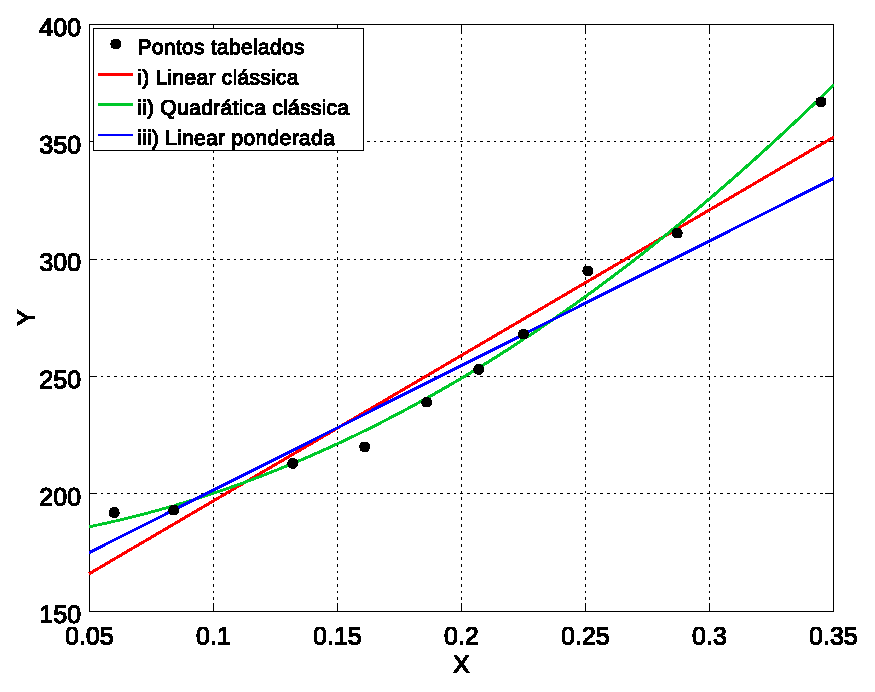
\includegraphics[width=0.80\linewidth]{I_fino}
		\captionsetup{width=0.80\linewidth}
		\caption{Diferentes funções aproximadoras dos pontos tabelados pelo critério dos mínimos quadrados clássico e ponderado.}
	\end{figure}

\newpage

\section{}
	\subsection{}
	\par
	Resposta no ficheiro \texttt{II/simpson.m}, corrido pelo \emph{script} \texttt{II/1.m}, onde é possível alterar o intervalo de integração, o número de subintervalos e a função a integrar.

	\subsection{}
	\subsubsection{}
	\par
	Correndo o programa \texttt{II/2.m}, obtém-se:
	$$F =  1480.56848008215$$

	\subsubsection{}
	\par
	Correndo o programa \texttt{II/2.m}, obtém-se:
	\begin{table}[H]
		\centering
		\begin{tabular}{|c|c|c|c|}
			\hline
			$n$	& $S_n$				& $|F - S_n|$		& $\frac{|F - S_n/2|}{|F - S_n|}$ \\ \hline
			2	& 1219.63999486000	& 260.92848522216	& -					\\ \hline
			4	& 1426.86928844946	& 53.69919163269	& 4.85907659480		\\ \hline
			8	& 1473.14779849473	& 7.42068158743		& 7.23642309672		\\ \hline
			16	& 1479.85678890922	& 0.71169117293		& 10.42682819413	\\ \hline
			32	& 1480.51545319880	& 0.05302688335		& 13.42132759730	\\ \hline
			64	& 1480.56497529815	& 0.00350478401		& 15.12985771736	\\ \hline
			128	& 1480.56825767195	& 0.00022241020		& 15.75819799559	\\ \hline
			256	& 1480.56846613061	& 0.00001395154		& 15.94162455869	\\ \hline
			512	& 1480.56847921284	& 0.00000086931		& 16.04897985126	\\ \hline
		\end{tabular}
		\caption{Comparação dos erros da regra de Simpson para vários valores de N.}
	\end{table}

	% TODO: comentar os erros
	% a majoração do erro depende de N quarticamente, por isso,
	% se N duplicar, o erro cai para 1/16.

\section{}
	\subsection{}
	\par %III- 1
	O programa desenvolvido tem o nome de \texttt{ponto\tu medio.m}. Recebe um intervalo
	$[a,b]$, uma função $f$ desenvolvida à parte, específica para cada problema de valor inicial, 
	uma condição inicial $ y_\alpha $ e um número $n$ de subintervalos.

	\subsection{}
		\subsubsection{}
		\par %III- 2
		Primeiramente, verifiquemos que o valor de $S$ para o qual $I(S) = 0$ é menor que 200.
		\par
		Isto pode ser feito com facilidade: olhando para $\frac{dI}{dS}$ conseguímos reparar que para valores
		de S inferiores a 300, tem valor com sinal constante. Logo, nesse intervalo, segundo o Teorema de Bolzano,
		há, no máximo, 1 zero. Como $[0, 200] \subset [0, 300]$, em $[0, 200]$ a derivada de I em função de S também não muda de sinal.
		Verificamos que há pelo menos um zero nesse intervalo por I(S) ser uma função contínua e por I(1) < 0 e I(200) > 0, 
		implicitando uma passagem pelo eixo das abcissas. Impondo a condição de ter que haver no mínimo uma passagem e ter que haver no máximo uma passagem, 
		podemos concluir que há um único zero no intervalo $[0, 200]$.
		\par
		Dividindo a segunda equação pela primeira, obtemos:
		
		% completar as Equações
		\begin{equation} \label{di}
		\begin{split}
			& \frac{dI}{dS} = -1 + \frac{300}{s}
			\Leftrightarrow dI = \left(-1 + \frac{300}{s}\right)dS   \\ 
			& \Leftrightarrow \frac{dI}{dt} dt = \left( -1 + \frac{300}{s}\right) \frac{dS}{dt} dt \\ 
			& \Leftrightarrow \int\frac{dI}{dt}dt = \int\left(\frac{-1 + 300}{s}\right)\frac{dS}{dt}dt =
			\int - \frac{ds}{dt}dt + \int\frac{300}{s}\frac{dS}{dt}dt \\
			& \Leftrightarrow I(t) = -S(t) + 300*log(S(t)) \\
		\end{split}
		\end{equation}

		Expressando $I(t)$ em função de $S(t)$, chegamos à equação que
		%aqui aquela que é para concluir)

		Impondo as condições iniciais:
		%isto mas menos cancerígeno:
		$$I(0) = -S(0) + 300* ln(S(0)) + c <=> c = bla bla bla$$


		O número máximo de crianças doentes num dado momento pode ser obtido
		atráves do máximo de $I(S)$. A sua derivada tem um único zero em $S = 300$,
		logo, sendo maior que 0 para valores inferiores a 300 e menor que 0 para valores superiores.
		Temos, portanto, um máximo em $S = 300$, que é também o máximo de $I(S)$ e que é
		o número de crianças suscetíveis quando o número de crianças infetadas é máximo.
		Substituindo na equação, obtemos:
		%Freitas... :)

		\subsubsection{}
		\par
		Se a epidemia acabar quando o número de crianças infetadas for 0, então, teremos
		que ver quantas crianças estão suscetíveis neste ponto, pois essas nunca serão infetadas, pelo menos nesta
		epidemia. Especialmente por ser varicela, uma doença que só se costuma ter uma vez,
		podemos ver que a transição de estados de uma criança
		é otimamente descrita por este diagrama.
		%lembras-te daquele diagrama de estados?...consegues?xD

		Uma criança, tirando a paciente zero, começa no estado suscetível. Passa
		para o estado infetado quando é infetada e depois de recuperada fica no estado de recuperada até ao fim da
		epidemia e provavelmente até ao fim da sua vida.

		%se não conseguires ou não te apetecer, é só preciso trocar algumas palavras

		Podia-se ter usado uma função que interpola polinómios já implementada.
		Em vez disso conseguímos um resultado igualmente satisfatório através de funções criadas por nós, pois
		quando o grupo foi avisado da existência e possibilidade de utilização de funções como $polynomial$ %era assim que se chamava, não era?
		já tinha tudo implementado.

		%consegues por + bonito:
		Quere-se um S tal que I(S) = 0 => S = I\^-1(0).
		A interpolação inversa consiste em aproximar a função inversa através de polinómios.
		Ao fazer-se isto, espera-se depois conseguir encontrar uma aproximação
		para a imagem de I\^-1(0), 
		que será o S que nós procuramos.
		\par
		Depois de utilizarmos as duas funções, concluímos que I\^-1(0) ~= 70.
		
		\subsubsection{}
		\par
		
		Utilizando a expressão $I(t) = -S(t) + 300 ln S(t) + c$ e substituindo
		os $I$ pelo lado direito da equação, obteremos uma equação na forma de um 
		PVI. A partir daí podemos usar o método do ponto médio para calcular aproximações $y_0$, $y_1$, ..., $y_N$ dos pontos
		$x_0$ = 0, $x_1$ = $x_0 + h$, ... $x_N= nh$ e desenhar o gráfico de acordo com esses pontos.
		
		Para obtermos um gráfico para o número de pessoas infetadas ao longo do tempo, usamos os nossos
		pontos já cálculados.
		Como I pode ser escrito em função de S ->
		I($x_i$) = -S($x_i$) + 300 * ln(S($x_i$) - 1205.
		
		Assim, para cada momento podemos saber uma aproximação do número de pessoas infetadas. E obtemos assim
		o gráfico da função I(t).
		
		Finalmente, para se conseguir fazer o gráfico de R foi necessário dividir a 3ª equação pela primeira e integrar:
		%contas, parecidas com a integração feita no 2-a. (escrevi a caneta nas folhas do freitas, mas já tinhamos feito igual)
		
		Ficamos com uma relação entre R(t) e S(t). Como temos aproximações para os S(t), 
		é-nos suficiente substituir as aproximações na expressão obtida e, assim, obter uma aproximação para R(t).
		
		Juntando os três gráficos:
		%gráfico(falta a imagem do gráfico freitas... fizeste push disso? :P)
		
		
		Relacionando o gráfico com o problema em questão, notamos que as aproximações feitas devem estar
		bastante próximas do valor certo/real de cada função, pois os gráficos comportaram-se e cumpriram as respetivas propriedades.
		
		
		%estou só a experimentar este itemize
		\begin{itemize}
		\item Como o limite superior de pessoas da amostra é 800, nenhuma função tem uma imagem acima de 800.
		\item O valor máximo para o número de pessoas infetadas num dado momento é 200 e tal pode-se confirmar pelo gráfico.
		\item Foi visto na pergunta $II.2-b)$ que o número de pessoas nunca infetadas é algo perto de 70. %verificar que é 70 certo ou nao...
		No gráfico, pode observar-se que Quando I(t) = 0, S(t) $\approx$ 70 e que fica constante nesse valor a partir do instante em que I(t) = 0.
		Faz todo o sentido ser constante a partir desse momento, porque quando se recupera a última pessoa infetada, deixa de haver probabilidades
		de se contrair varicela e a partir daí o número de pessoas suscetíveis, isto é, que nunca contrairam varicela, é constante.
		\item Em termos de interpretação do problema, o formato do gráfico da função das pessoas recuperadas assenta nas interpretações
		feitas sobre o problema.
		Se deixam de haver infetados a partir de determinado momento, 
		também a partir desse momento deveriam parar de haver recuperados.
		Além disso, o número de recuperados nunca deve diminuir pois estes nunca mais voltam a ser infetados. A varicela é assim.
		\end{itemize}
		

\end{document}
